\documentclass[a4paper,UTF8]{ctexart}

\usepackage{amsmath, amsthm, amssymb, amsfonts, hyperref, mathrsfs}%美国数学学会的包+?
\usepackage{geometry} %控制界面
\usepackage{bookmark}
\usepackage{fancyhdr} % header & footer
\usepackage{appendix} % 附录
\usepackage{tikz} %作图
\usepackage{graphicx} %插入图片的宏包
\usepackage{float} %设置图片浮动位置的宏包
\usepackage{subfigure} %插入多图时用子图显示的宏包
\usepackage{listings} %引用代码
\usepackage{physics,mathtools} %物理数学工具
\usepackage{framed}
\geometry{top=2.5cm,bottom=2.5cm,left=2.5cm,right=2.5cm} % 布局要求
\pagestyle{fancy} % fancy分格
\fancyhf{} % 清除所有页眉页脚
\renewcommand\headrulewidth{0.6pt}
\renewcommand\footrulewidth{0.6pt}
\lhead{何金铭 PB21020660$\mid$座位号:4}
\chead{弗兰克-赫兹实验实验报告}
\rhead{\thepage}
%\lfoot{2022.11.10}
%\rfoot{USTC}
\bibliographystyle{plain} % 引用样式
\everymath{\displaystyle} % display
%============================================================

\begin{document}

\begin{center}
    \textbf{\Large 弗兰克-赫兹实验实验报告}
    \par \text{\large 何金铭 PB21020660}
\end{center}

\section{实验目的}

1.通过测定氩原子等元素的第一激发电位,证明原子能级的存在。

2.了解电子与原子碰撞和能量交换过程的微观图象

3.了解研究原子内部能量问题时所采用的基本实验方法。

4.进一步理解玻尔的原子理论

\section{实验原理}

夫兰克一赫兹实验原理(如图 1 所示),氧化物阴极 K,阳
极 P,第一、第二栅极分别为 G1、G2。
K-G1-G2 加正向电压,为电子提供能量。UG1K 的作用主要是
消除空间电荷对阴极电子发射的影响,提高发射效率。G2-P 加
反向电压,形成拒斥电场。
电子从 K 发出,在 K-G2 区间获得能量,如果电子进入 G2-P
区域时动能大于或等于 $eU_{G2P}$,就能到达板极形成板极电流 $I$.

\begin{figure}[H]
    \centering
    \begin{minipage}[b]{0.45\textwidth}
        \centering
        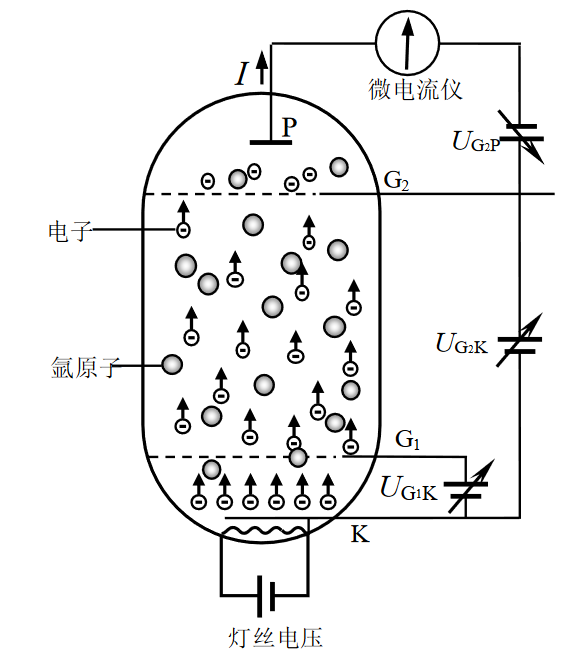
\includegraphics[width=0.8\textwidth]{./fh_app.png}
        \caption{弗兰克-赫兹实验原理图}
    \end{minipage}
    \begin{minipage}[b]{0.45\textwidth}
        \centering
        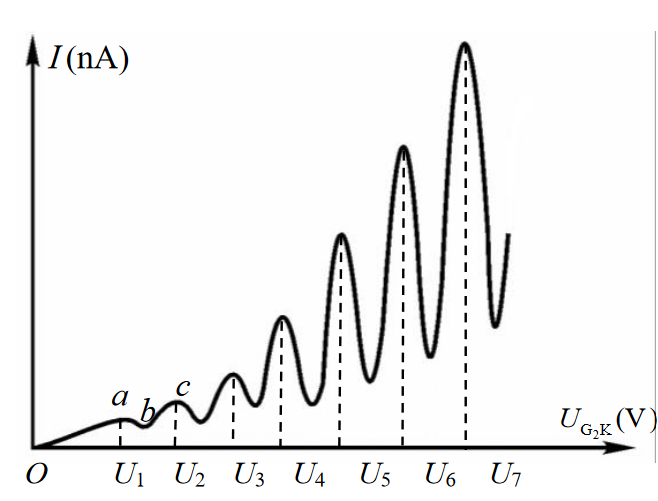
\includegraphics[width=0.8\textwidth]{./fh_fig.png}
        \caption{弗兰克-赫兹实验$V_{G_{2}K} \sim I$曲线}
    \end{minipage}
\end{figure}

\begin{enumerate}
    \item {\bfseries{$K$-$G_{1}$区间}} 电子迅速被电场加速而获得能量。
    \item {\bfseries{$G_{1}$-$G_{2}$区间}} 电子继续从电场获得能量并不断与氩原子碰撞。当其能量小于氩原子第一
激发态与基态的能级差$\Delta E = E_{2}-E_{1}$时,氩原子基本不吸收电子的能量,碰撞属于弹性碰撞。当电子
的能量达到$\Delta E$,则可能在碰撞中被氩原子吸收这部分能量,这时的碰撞属于非弹性碰撞。$\Delta E$称为
临界能量。
    \item {\bfseries{$G_{2}$-P区间}} 电子受阻,被拒斥电场吸收能量。若电子进入此区间时的能量小于 eUG2P 则
不能达到板极。
\end{enumerate}

由此可见,若 $e U_{G2K}<\Delta E$,则电子带着$e U_{G2K}$的能
量进入 $G_{2}$-P 区域。随着 $G_{G2K}$ 的增加,电流$I$ 增加(如
图 2 中 $Oa$ 段)。

若 $e U_{G2K}=\Delta E$ 则电子在达到 $G_2$ 处刚够临界能量,
不过它立即开始消耗能量了。继续增大 $U_{G2K}$,电子能
量被吸收的概率逐渐增加,板极电流逐渐下降(如图
2 中 $ab$ 段)。

继续增大 $U_{G2K}$,电子碰撞后的剩余能量也增加,
到达板极的电子又会逐渐增多(如图 2 中 $bc$ 段)。

若 $e U_{G2K}>\Delta E$ 则电子在进入 $G_2$-P 区域之前可能 $n$ 次被氩原子碰撞而损失能量。板极电流 $I$ 随加
速电压 $U_{G2K}$ 变化曲线就形成 $n$ 个峰值,如图 2 所示。相邻峰值之间的电压差
$\Delta U$ 称为氩原子的第一
激发电位。氩原子第一激发态与基态间的能级差

\begin{equation}
    \Delta E = e \Delta U
\end{equation}

\section{实验仪器}

微机型弗兰克一赫兹实验仪(FD-FH-C),示波器

\section{实验内容}

\subsection{用示波器观察氩原子的激发曲线}

\subsection{测量氩原子的激发曲线}

\section{测量记录}

\subsection{用示波器观察氩原子的激发曲线}

\subsubsection{$U_F$、$U_{G1k}$、$U_{G2K}$、$U_{G2P}$参考值记录}

\begin{table}[htb]
    \begin{center}
        \begin{tabular}{|c|c|c|c|c|}
            \hline
            \bfseries 参考参数 & $V_F$ & $V_{G1}$ & $V_P$ & $V_{G2}$ \\
            \hline
            \bfseries $V$ & 2.50 & 1.50 & 9.80 & 0-100 \\
            \hline
        \end{tabular}
    \end{center}
    \caption{$U_F$、$U_{G1k}$、$U_{G2K}$、$U_{G2P}$参考值}
\end{table}

\subsubsection{调节$U_F$、$U_{G1k}$、$U_{G2K}$、$U_{G2P}$,并描述各实验参数对激发曲线的影响,分析各参数对激发曲线的作用机制}

%\begin{framed}
{\uppercase\expandafter{\romannumeral 1}  \bfseries $U_{F} \quad 1.25V \longrightarrow 3.75V$}
%\end{framed}
\begin{framed}
\begin{enumerate}
    \item 从$2.5V$到$1.25V$时,曲线的峰值开始下降,最终趋于一条直线,并不停的有抖动。
    \item 当从$1.25V$到$2.1V时$,曲线开始恢复之前的峰的状态,虽然高度不如之前,并且这一过程中存在一定时间间隔。
    \item 当从$2.10V$到$2.50V$时,曲线开始纵向伸长,且最终曲线高度高于原曲线高度。
    \item 当从$2.50V$到$3.75V$时,曲线的高度不断变化,此时调节示波器,发现当电压到达一定值时,曲线达到最高处(示波器无法显示),
    此时峰值开始消失,变为直线;当到达$3.75V$时,峰值完全消失,变为一条直线。
\end{enumerate}
\end{framed}

{\uppercase\expandafter{\romannumeral 2} \bfseries $U_{G_{1}K} \quad 0.75V \longrightarrow 2.25V$}

\begin{framed}
\begin{enumerate}
    \item 从$0.75V$到$1.50V$时,峰值之间的高度差逐渐变小。
    \item 从$1.50V$到$2.25V$时,峰值之间的高度差进一步变小,图像更加平缓。
\end{enumerate}    
\end{framed}

{\uppercase\expandafter{\romannumeral 3} \bfseries $U_{G_{2}K} \quad 0 \longrightarrow 100 V$}

\begin{framed}
\begin{enumerate}
    \item $U_{G_{2}K}< 5.7V$时,波形完全消失,变为一条小线段。
    \item 从$5.7V$变为$9.6V$时,出现了第一个波峰
    \item 从$9.6V$变为$12V$时,出现了第一个波谷
    \item 以此类推,当电压增加的时候,逐渐出现更多的波峰波谷,直至电压最大时,出现了7个波峰波谷。
\end{enumerate}    
\end{framed}

{\uppercase\expandafter{\romannumeral 4} \bfseries $U_{G_{2}P} \quad 4.9V \longrightarrow 14.7V$}

\begin{framed}
    \begin{enumerate}
        \item 从$4.9V$到$9.8V$时,整体电流波形高度下降,且波峰波谷之间的差值变大,大致形状相似
        \item 从$9.8V到14.7V$时,整体电流波形高度继续下降,但波峰波谷之间的差值变小,且当电压调至$14.7V$时
        第一个波峰近乎水平,其余的波峰波谷也变得极其扁平。
    \end{enumerate}
\end{framed}

\subsection{测量氩原子的激发曲线}

\subsubsection{粗测峰、谷数据}

\begin{table}[!htp]
    \centering
    \begin{tabular}{|c|c|c|c|c|c|c|c|}
    \hline
        实验次数 & 1 & 2 & 3 & 4 & 5 & 6 & 7 \\ \hline
        峰值电压/V & 17.8 & 28.1 & 38.7 & 49.6 & 61.2 & 73.0 & 85.7  \\ \hline 
        谷值电压/V & 23.0 & 33.6 & 44.3 & 55.4 & 66.8 & 78.9 & 91.3   \\ \hline
    \end{tabular}
    \caption{6组峰值谷值粗测}
\end{table}

\subsubsection{测量6个完整的峰、谷数据}

\newpage

\begin{table}[H]
    \centering
    \begin{tabular}{|c|c|c|c|c|c|c|c|c|}
    \hline
        实验次数 & $U/V$ & $I_{P}/0.1 \mu A$ & 实验次数 & $U/V$ & $I_{P}/0.1 \mu A$ & 实验次数 & $U/V$ & $I_{P}/0.1 \mu A$ \\ \hline
        1 & 10 & 0.073 & 20 & 26 & 0.76 & 39 & 39.5 & 1.208 \\ \hline
        2 & 11 & 0.081 & 21 & 27 & 0.876 & 40 & 40 & 1.113 \\ \hline
        3 & 12 & 0.141 & 22 & 27.5 & 0.9 & 41 & 41 & 0.851 \\ \hline
        4 & 13 & 0.219 & 23 & 28 & 0.904 & 42 & 42 & 0.537 \\ \hline
        5 & 14 & 0.304 & 24 & 28.5 & 0.885 & 43 & 43 & 0.261 \\ \hline
        6 & 15 & 0.382 & 25 & 29 & 0.847 & 44 & 43.5 & 0.184 \\ \hline
        7 & 16 & 0.421 & 26 & 30 & 0.69 & 45 & 44 & 0.167 \\ \hline
        8 & 17 & 0.462 & 27 & 31 & 0.487 & 46 & 44.5 & 0.243 \\ \hline
        9 & 17.5 & 0.461 & 28 & 32 & 0.298 & 47 & 45 & 0.391 \\ \hline
        10 & 18 & 0.46 & 29 & 33 & 0.182 & 48 & 45.6 & 0.61 \\ \hline
        11 & 19 & 0.445 & 30 & 33.5 & 0.198 & 49 & 46 & 0.772 \\ \hline
        12 & 20 & 0.4 & 31 & 34 & 0.287 & 50 & 47 & 1.126 \\ \hline
        13 & 21 & 0.337 & 32 & 35 & 0.57 & 51 & 48 & 1.41 \\ \hline
        14 & 22 & 0.265 & 33 & 36 & 0.904 & 52 & 48.5 & 1.494 \\ \hline
        15 & 22.5 & 0.244 & 34 & 37 & 1.145 & 53 & 49.1 & 1.535 \\ \hline
        16 & 23 & 0.246 & 35 & 37.5 & 1.217 & 54 & 49.5 & 1.555 \\ \hline
        17 & 23.5 & 0.286 & 36 & 38 & 1.269 & 55 & 50 & 1.536 \\ \hline
        18 & 24 & 0.359 & 37 & 38.5 & 1.273 & 56 & 50.6 & 1.47 \\ \hline
        19 & 25 & 0.562 & 38 & 39 & 1.257 & 57 & 51 & 1.393 \\ \hline
        实验次数 & $U/V$ & $I_{P}/0.1 \mu A$ & 实验次数 & $U/V$ & $I_{P}/0.1 \mu A$ & 实验次数 & $U/V$ & $I_{P}/ \mu A$ \\ \hline
        58 & 52 & 1.1 & 80 & 67.1 & 0.584 & 102 & 84.2 & 0.274 \\ \hline
        59 & 53 & 0.76 & 81 & 67.6 & 0.692 & 103 & 84.8 & 0.278 \\ \hline
        60 & 54 & 0.432 & 82 & 68 & 0.816 & 104 & 85.3 & 0.281 \\ \hline
        61 & 54.5 & 0.31 & 83 & 69.1 & 1.201 & 105 & 86 & 0.28 \\ \hline
        62 & 55.6 & 0.318 & 84 & 70 & 1.477 & 106 & 86.5 & 0.276 \\ \hline
        63 & 56 & 0.455 & 85 & 71 & 1.733 & 107 & 87.1 & 0.267 \\ \hline
        64 & 56.5 & 0.644 & 86 & 72 & 1.892 & 108 & 88 & 0.249 \\ \hline
        65 & 57 & 0.841 & 87 & 72.5 & 1.934 & 109 & 89 & 0.226 \\ \hline
        66 & 58.1 & 1.207 & 88 & 73.1 & 1.943 & 110 & 90.1 & 0.209 \\ \hline
        67 & 59 & 1.473 & 89 & 73.7 & 1.913 & 111 & 90.8 & 0.205 \\ \hline
        68 & 60 & 1.67 & 90 & 74.3 & 1.841 & 112 & 91.5 & 0.208 \\ \hline
        69 & 60.5 & 1.724 & 91 & 75 & 1.689 & 113 & 91.8 & 0.212 \\ \hline
        70 & 61 & 1.749 & 92 & 76 & 1.418 & 114 & 92.3 & 0.218 \\ \hline
        71 & 61.5 & 1.736 & 93 & 77 & 1.114 & 115 & 92.7 & 0.225 \\ \hline
        72 & 62 & 1.69 & 94 & 77.6 & 0.988 & 116 & 93.1 & 0.234 \\ \hline
        73 & 62.5 & 1.61 & 95 & 78.2 & 0.907 & 117 & 93.7 & 0.246 \\ \hline
        74 & 63 & 1.495 & 96 & 78.8 & 0.911 & 118 & 94.2 & 0.256 \\ \hline
        75 & 64 & 1.187 & 97 & 79.7 & 1.027 & 119 & 94.9 & 0.272 \\ \hline
        76 & 65 & 0.832 & 98 & 80.3 & 1.189 & 120 & 95.1 & 0.275 \\ \hline
        77 & 65.6 & 0.648 & 99 & 81 & 1.364 & ~ & ~ & ~ \\ \hline
        78 & 66.1 & 0.544 & 100 & 82 & 1.65 & ~ & ~ & ~ \\ \hline
        79 & 66.7 & 0.53 & 101 & 83.1 & 1.88 & ~ & ~ & ~ \\ \hline
    \end{tabular}
    \caption{原始数据}
\end{table}

\newpage

\section{分析与讨论}

\subsection{分析$U_F$、$U_{G1k}$、$U_{G2K}$、$U_{G2P}$实验参数变化对激发曲线的影响,并分析其对激发曲线的作用机制}

总结一下在实验记录中的语言:

\begin{description}
    \item[\bfseries $U_{F} \quad 1.25V \longrightarrow 3.75V$] $U_F$增加时,曲线整体拉伸,各部位比例基本一致,最终超过示波器量程。
    \item[\bfseries $U_{G_{1}K} \quad 0.75V \longrightarrow 2.25V$] $U_{G_{1}K}$增加时,曲线峰值间的高度差逐渐减小。
    \item[\bfseries $U_{G_{2}K} \quad 0 \longrightarrow 100 V$] $U_{G_{2}K}$增加时,曲线的波峰波谷数目增加
    \item[\bfseries $U_{G_{2}P} \quad 4.9V \longrightarrow 14.7V$] $U_{G_{2}P}$增加时,曲线的整体波形高度下降,且峰谷间距先增大后减小。
\end{description}

\subsection{查阅资料,分析原因}

%\begin{framed}
{\uppercase\expandafter{\romannumeral 1}  \bfseries $U_{F}$} 现象于实验记录中有写\cite{UF}
%\end{framed}
\begin{framed}
阴极电压$U_F$很小的时候, 板极电流$I_P$起伏不大, 这是由于阴极电压$U_F$小了阴极就只能发射出少量的电子,
 进而参与非弹性碰撞的电子和到达板极的电子就少了。所以板极电流$I_P$的大小起伏变化不大。
 随着阴极电压$U_F$逐渐增大, 板极电流$I_P$的大小起伏也变大, 这是由于阴极电压Uk大了阴极发射出大量的电子, 
 参与非弹性碰撞的电子就多, 到达板极的电子也多了。所以板极电流$I_P$的大小起伏也变大。
\end{framed}

{\uppercase\expandafter{\romannumeral 2} \bfseries $U_{G_{1}K}$} {\textbf{调研现象:}}随着$U_{G_{1}K}$的增大,峰谷电流呈现先急剧增大,而后波动式递减的规律。\cite{UG1K}

\begin{framed}

由于观察到的现象只是抑制的部分,这里只给出抑制的原因。

抑制机理:后期峰谷电流大小随$U_{G_{1}K}$增大而总体递减当$U_{G_{1}K}$继续增大时,峰谷电流大小呈现总体递减的趋势。

\begin{enumerate}
    \item 当$U_{G_{1}K}$进一步增大时,阴极K发射的热电子获得的初动能也进一步增大。根据冉绍尔-汤森效应,在电子-氩气体系中,当电子能量介于1~10 $eV$之间时,氩原子的总碰撞截面随电子能量升高而单调递增,故电子与氩原子在$KG_{1}$区域的弹性碰撞能损也将增大,导致发射电子能量降低,进而降低板极电流$I_{A}$,从而同步降低其峰谷值。
    \item 由机理3可得,热电子与氩原子在$KG_1$区域的弹性碰撞能损将增大,氩气温度将升高。根据文献的研究结论,当氩气压强处于一个大气压,温度在200~500 $K$变化时,其热导率将随温度升高而增大。电子与氩原子的碰撞使阴极K附近的氩气局部温度升高,导热性增强,使得灯丝的散热速率加大;而灯丝电压不变、功率不变、产热速率不变,故灯丝将进入散热速率大于产热速率的过渡态。当灯丝达到新的热平衡态时,其温度应当降低。而由Richardson-Dushman方程,灯丝温度直接决定了发射电流密度的大小。换言之,当灯丝温度降低时,发射电流密度将显著减小,从而同步降低峰谷电流。
\end{enumerate}    
\end{framed}

{\uppercase\expandafter{\romannumeral 3} \bfseries $U_{G_{2}K}$} 提高加速电压UG2K的上限, 能够得到更多的波峰波谷\cite{U2}

\begin{framed}
\begin{enumerate}
    \item 当 加 速电 压 $U_{G_{2}K}$达 到 氩 原子 的 第一 激 发电位 $U_0$时,
    由于阴极 发射电子的速率 符合 麦克 斯韦分布
函数,此 时 氩 原子就会首先 和最 大 速率 $V_{max}$ 的电子 进行 非
弹性碰撞,此时电子把自身的动能全部交给氩原子实现从基
态到第一激 发态的跃 迁,此时电流 开始下降,第一个 峰值电
流形成。随着加速电压的增加,从阴极发射出来的其他速率
的电子的动能也陆续 到达氩 原子从 基态 跃 迁 到第一激 发 态
时需要的能量,这部分电子就会把自己的动能全部交给氩原子实现 跃迁,所以不能到达极板的电子的数目会越来越多,
当速率最小的电子 $V_{min}$ 的动能达到氩原子跃迁到第一激发电
位时所需要的能量时,这部分电子把自身的动能全部交给氩
原子实现 跃 迁,因此不能到达极板的电子的数目达到最多,
第一谷值电流形成。
    \item 电压继续增大,当加速电压$U_{G_{2}K}=2U_0$时,从阴极发射
出来的最 大 速率的电子就会 和两个不同的处 于基态的氩 原
子实现两次非弹性碰撞,最终通过两次碰撞后把自身的动能
全 部交 给了氩 原子,能 够 到达极板 的电子的 数目会减 少,所
以电流 开始下降,这就 是第二个峰的形成。当加速电压 继续
增 大 时,其他 速率 的电子 的动 能 也 陆续 到达 和 氩 原子 碰 撞
两次时所需要的能量,此时能够到达极板的电子的数目也减
少,当从阴极发射出来的最小速率的电子的动能达到与氩原子碰撞两次所需 能量时,电流 达到最小值,这就是第二个谷
的形成。
    \item 对于加速电压继
续增大时峰谷形成的原因与上面分析类似。
\end{enumerate}    
\end{framed}

{\uppercase\expandafter{\romannumeral 4} \bfseries $U_{G_{2}P}$} \cite{UF}

\begin{framed}
    \begin{enumerate}
        \item 反向电压给发生非弹性碰撞而损失大量能量的电子施以一个适当的力, 而电子因仅剩少量能量而无法克服这个反向电压到达板极, 进而使得板极电流$I_P$明显下降。
        \item 增加反向电压后发现板极电流$I_P$的起伏越来越明显。这是由于反向电压控制着发生非弹性碰撞的电子到达板极, 因而板极电流$I_P$的起伏就很明显。继续增加反向电压发现, 板极电流$I_P$反而越来越小夫兰克-赫兹曲线下移,反向电压越大电子速度就越小, 单位时间内到达板极的电子就越少。
    \end{enumerate}
\end{framed}

\subsection{绘制氩原子的激发曲线}

\subsubsection{绘制激发曲线}

利用三次样条插值,程序运用了scipy.interpolate.CubicSpline()函数,给出了氩原子的激发曲线:

\begin{figure}[H]
    \centering
    \begin{minipage}[b]{0.9\textwidth}
        \centering
        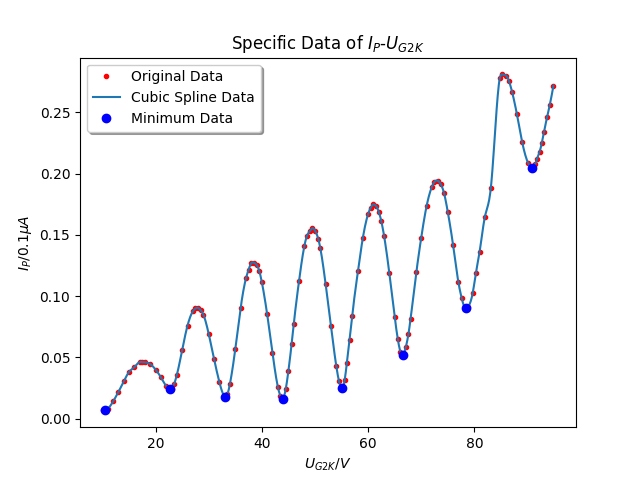
\includegraphics[width=0.7\textwidth]{./cs.png}
        \caption{氩原子激发曲线}
    \end{minipage}
\end{figure}

\subsection{绘制激发曲线的包络线}

假设曲线的包络线方程满足:

\begin{equation}
    y = a \cdot e^{b\cdot x} + c
\end{equation}

下面利用了曲线拟合,程序运用了scipy.optimize.curve$\_$fit()函数,做出了包络线。

并且给出了曲线参数:

\begin{equation}
    \left\{
        \begin{aligned}
            a=3\times 10^{-11}A & &\\
            b=7.1\times 10^{-2} V^{-1} & &\\
            c = 1.3\times 10^{-9}A & &
        \end{aligned}\right.
\end{equation}

\begin{figure}[H]
    \centering
    \begin{minipage}[b]{0.9\textwidth}
        \centering
        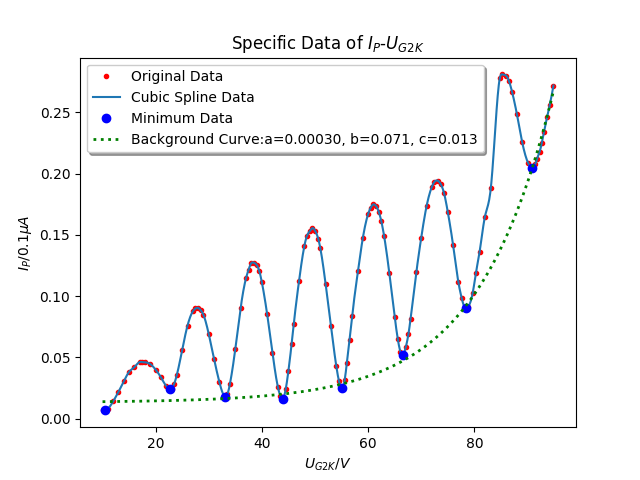
\includegraphics[width=0.7\textwidth]{./back.png}
        \caption{氩原子激发曲线的包络线}
    \end{minipage}
\end{figure}

\subsubsection{绘制相差曲线}

将原曲线减去包络线,即可得到相差曲线。

\begin{figure}[H]
    \centering
    \begin{minipage}[b]{0.9\textwidth}
        \centering
        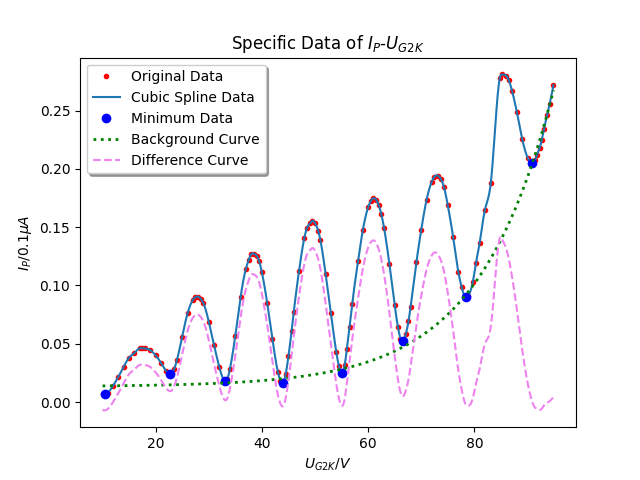
\includegraphics[width=0.7\textwidth]{./difference.png}
        \caption{氩原子激发曲线的相差曲线}
    \end{minipage}
\end{figure}

\subsubsection{计算氩原子的第一激发电位,并计算A类不确定度}

对于求得的差异曲线,认为单个峰值曲线是轴对称的,故可以利用程序进行查找,
找到第k个曲线左右的$50\%$高度的点的电压值$U_{k , left}$和$U_{k , right }$,
将其求平均值,即可得峰值的电压值$U_k = \frac{U_{k , left}+U_{k , right }}{2}$。

于是得到数据:

\begin{table}[!htp]
    \centering
    \begin{tabular}{|c|c|c|c|c|c|c|c|}
    \hline
        峰值数 & 1 & 2 & 3 & 4 & 5 & 6 & 7 \\ \hline
        $U_{G_{2}K}/V$ & 17.15 & 27.85 & 38.45 & 49.40 & 60.75 & 72.55 & 85.80 \\ \hline
    \end{tabular}
    \caption{峰值处的电势值表}
\end{table}

于原图中绘制出,则有:

\begin{figure}[H]
    \centering
    \begin{minipage}[b]{0.9\textwidth}
        \centering
        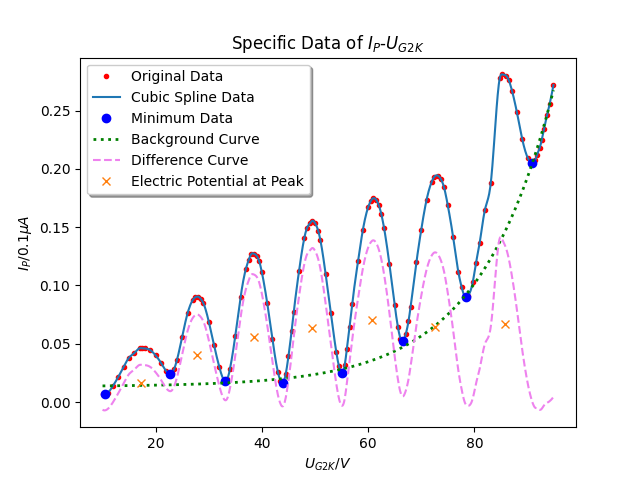
\includegraphics[width=0.7\textwidth]{./peak.png}
        \caption{峰值处的电势值}
    \end{minipage}
\end{figure}


最小二乘法作图如下:

\begin{figure}[H]
    \centering
    \begin{minipage}[b]{0.9\textwidth}
        \centering
        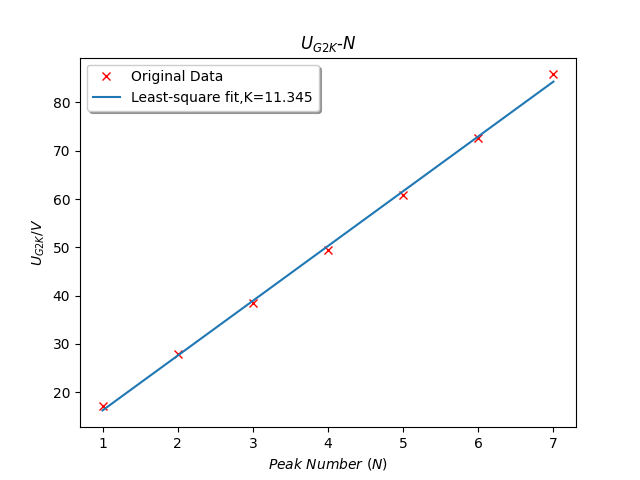
\includegraphics[width=0.7\textwidth]{./ls.png}
        \caption{$U_{G_{2}K}$-$N$关系图}
    \end{minipage}
\end{figure}

在最小二乘法中,对于$N$组点的拟合,有以下约定:

\begin{equation}
    \varepsilon_i = (y_i - a - b x_i)
\end{equation}

\begin{equation}
    \Delta = N \sum(x^2) - (\sum x)^2
\end{equation}

经过最小二乘法处理可得:斜率$K=11.345$。

其不确定度的计算公式为:

\begin{equation}
    \sigma_K = \sqrt{\frac{1}{N-2} \sum_{i=1}^{N}\varepsilon_i^{2} \cdot \frac{N}{\Delta}} = 0.19
\end{equation}

所以有:

\begin{equation}
    K = 11.345 \pm 0.19
\end{equation}

斜率就是我们要求的氩原子第一激发电位$U_0$

有:

\begin{equation}
    U_0 = 11.345 V \pm 0.19V
\end{equation}

\subsection{误差分析与总结}

\subsubsection{误差分析}

下面进行误差分析

\begin{enumerate}
    \item 实验的主要误差来自于操作时记录数据的时间间隔,由于在记录数据的时候,电流$I_P$也会随之衰减,不同的记录间隔可能导致$I_P$的误差。
    \item 在实验的过程中,由于电流示数超过量程,还进行了一次电流表的量程的切换,在这个过程中也会带来一定的误差。
    \item 还可能存在一些仪器的固有误差。
\end{enumerate}

\subsubsection{总结}

\begin{enumerate}
    \item 最终测得$U_0 = 11.345 V \pm 0.19V$,其与理论值$11.50V$较为接近,且在相对不确定度为$1.7\%$,在$5\%$之内,可以接受。
\end{enumerate}

\section{思考题与课间计算}

\subsection{计算 80、90、100、160、170、180°C时电子在汞蒸汽中的平均自由程$\lambda$}

已知在汞蒸汽中电子的平均自由程$\lambda$与温度 $T$、蒸汽压 $p$ 的关系为:

\begin{equation}
    \lambda  = \frac{KT}{\pi r^2 p}
\end{equation}

代入数据即可算得:

\begin{table}[!htp]
    \centering
    \begin{tabular}{|c|c|c|c|c|c|c|}
    \hline
        $T/ ^\circ C$ & 80 & 90 & 100 & 160 & 170 & 180  \\ \hline 
        $\lambda / m$ & $4.24 \cdot 10^{-3}$ & $2.43 \cdot 10^{-3}$ & $1.45 \cdot 10^{-3}$ & $1.10 \cdot 10^{-4}$ & $7.69 \cdot 10^{-5}$ & $5.48\cdot 10^{-5}$   \\ \hline
    \end{tabular}
    \caption{电子在汞蒸气中六个温度时的平均自由程}
\end{table}

\subsection{$U_{G2K} \sim I_{p}$曲线电流下降并不十分陡峭,主要原因是什么?}

下降不陡峭,说明到达P极的电子仍然存在,主要原因有以下:

\begin{enumerate}
    \item 吸收了电子的氩原子处于高能级状态,根据量子力学,系统哈密顿量越大,其跃迁至低能级的概率越大,故
    氩原子容易发生二次激发电子,使得仍有部分电子可以到达P极
    \item 电子的电场可能会使得部分氩原子电离,使得电子发生散射,减少了吸收电子的数量
    \item 也可能有部分电子不会被氩原子吸收
\end{enumerate}

\subsection{$I$ 的谷值并不为零,而且谷值依次沿$U_{G_{2}K}$轴升高,如何解释?}

$I$的谷值不为零的原因和上一题类似,在此不重复说明。谷值依次沿$U_{G_{2}K}$轴升高的原因有:

\begin{enumerate}
    \item 主要原因是:继续增大 $U_{G2K}$,电子碰撞后的剩余能量也增加,
到达板极的电子又会逐渐增多
    \item 次要原因是:当电压增大的时候,氩原子的二次激发更加容易,氩原子更容易发生电离,电子穿透氩原子的概率也会增大,故谷值上升。
\end{enumerate}

\subsection{第一峰值所对应的电压是否等于第一激发电位?原因是什么?}

不等于,因为存在一个漂移电压$U_{G_{1}K}$,故它们之间至少相差一个漂移电压;
并且也可能会存在其他的原因影响。

\subsection{写出氩原子第一激发态与基态的能级差。}

由能量守恒可得:

\begin{equation}
    \Delta E = e \Delta U
\end{equation}

其中,$\Delta U$为氩原子的第一激发电位,$e$为电子元电荷量

% 参考文献

\bibliography{math}

% 结束文档

\end{document}